\chapter{Synchronisation: Locks, Barriers and Coordination}\label{ch:sync}
\begin{center}\small\textit{Many threads, one memory: how to take turns without colliding or starving.}\end{center}

\begin{quote}
\emph{``A race is not who finishes first, but whether the result depends on who did.''} Without synchronisation, the same program can give different answers on different runs.
\end{quote}

\noindent\fbox{\parbox{\dimexpr\linewidth-2\fboxsep-2\fboxrule}{%
\textbf{From zero: why threads must coordinate.} We start with a single thread and shared data, show how interleavings create races, then build the ladder of primitives: mutual exclusion, spinlocks and queue locks, read--write locks, semaphores, and barriers. Every mechanism is motivated by a failure it fixes.}}
\vspace{0.4em}

\section*{Learning Outcomes}
After this chapter you will be able to:
\begin{enumerate}[label=(L\arabic*)]
    \item define race condition, critical section and mutual exclusion with an interleaving proof;
    \item implement and compare spinlocks (test-and-set, test-and-test-and-set, MCS) on contention and traffic;
    \item distinguish read--write locks, semaphores and monitors and choose among them;
    \item explain centralised, dissemination and tree barriers and their step complexity;
    \item detect deadlock, livelock and convoying and apply remedies (ordering, backoff, combining).
\end{enumerate}

% ============================================================
\section{The Race Problem}\label{sec:race}
A \emph{race condition} occurs when correctness depends on the interleaving of concurrent accesses to shared data without ordering. Consider two threads each doing \texttt{counter++}, which compiles to load--add--store. With initial \texttt{counter}=0, the interleaving load0, load0, add, add, store1, store1 leaves counter as 1 instead of 2. The operations are not atomic.

\begin{definition}[Critical section and mutual exclusion]
A \emph{critical section} (CS) is a code region that accesses shared state requiring atomicity. \emph{Mutual exclusion} guarantees at most one thread executes its CS at a time. Progress and bounded waiting add liveness: some thread eventually enters, and no thread starves forever.
\end{definition}

The fix is to bracket the CS with \texttt{acquire} and \texttt{release} of a lock. The lock's protocol must itself be race-free, using an atomic hardware primitive.

\begin{center}
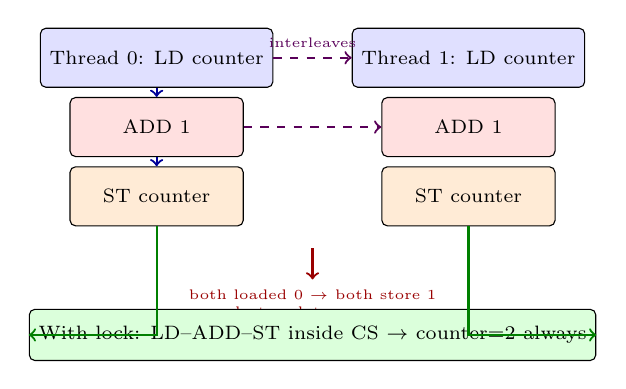
\begin{tikzpicture}[font=\scriptsize, scale=0.88]
\node[draw, fill=blue!12, minimum width=2.2cm, minimum height=0.75cm, rounded corners=2pt] (t0) at (0,2.2) {Thread 0: LD counter};
\node[draw, fill=blue!12, minimum width=2.2cm, minimum height=0.75cm, rounded corners=2pt] (t1) at (4.5,2.2) {Thread 1: LD counter};
\node[draw, fill=red!12, minimum width=2.2cm, minimum height=0.75cm, rounded corners=2pt] (a0) at (0,1.2) {ADD 1};
\node[draw, fill=red!12, minimum width=2.2cm, minimum height=0.75cm, rounded corners=2pt] (a1) at (4.5,1.2) {ADD 1};
\node[draw, fill=orange!16, minimum width=2.2cm, minimum height=0.75cm, rounded corners=2pt] (s0) at (0,0.2) {ST counter};
\node[draw, fill=orange!16, minimum width=2.2cm, minimum height=0.75cm, rounded corners=2pt] (s1) at (4.5,0.2) {ST counter};
\draw[->, thick, blue!60!black] (t0) -- (a0);
\draw[->, thick, blue!60!black] (a0) -- (s0);
\draw[->, thick, violet!70!black, dashed] (t0.east) -- (t1.west) node[midway, above, font=\tiny] {interleaves};
\draw[->, thick, violet!70!black, dashed] (a0.east) -- (a1.west);
\draw[->, thick, red!60!black] (2.25,-0.55) -- (2.25,-1.0) node[below, font=\tiny, align=center] {both loaded 0 $\to$ both store 1\\lost update = race};
\node[draw, fill=green!14, minimum width=5.8cm, minimum height=0.65cm, rounded corners=2pt] (fix) at (2.25,-1.8) {With lock: LD--ADD--ST inside CS $\to$ counter=2 always};
\draw[->, thick, green!50!black] (s0.south) |- (fix.west);
\draw[->, thick, green!50!black] (s1.south) |- (fix.east);
\end{tikzpicture}
\end{center}

Peterson's algorithm solves mutual exclusion for two threads with only loads/stores but is subtle and not scalable. Modern hardware provides \texttt{atomic} read-modify-write: \texttt{test-and-set}, \texttt{fetch-and-add}, \texttt{compare-and-swap (CAS)}.

% ============================================================
\section{Spinlocks: From Simple to Scalable}\label{sec:spinlocks}
A \emph{spinlock} busy-waits until the lock is free. The minimal primitive is \texttt{test-and-set}: atomically set lock to 1 and return old value; 0 means success.

Naive CAS every iteration invalidates the line each time, hammering the interconnect. \emph{Test-and-test-and-set (TTAS)} first spins on a cached read (state S, no traffic) and only attempts CAS when the lock appears free. This reduces traffic from $O(P)$ per spin to near zero in the common case.

TTAS still suffers convoying: when the holder releases, all spinners thunder and one CAS storm occurs. \emph{Queue locks (MCS, CLH)} eliminate it: each thread enqueues a node and spins on its \emph{own} line. Handover is $O(1)$ and local.

\begin{center}
\begin{tikzpicture}[font=\scriptsize, scale=0.88]
\node[draw, fill=blue!14, minimum width=1.5cm, minimum height=0.75cm, rounded corners=2pt, align=center] (head) at (0,0) {Queue tail\\{\tiny atomic SWAP}};
\node[draw, fill=green!14, minimum width=1.3cm, minimum height=0.75cm, rounded corners=2pt, align=center] (n0) at (2.6,0) {T0 qnode\\{\tiny locked=0}};
\node[draw, fill=orange!16, minimum width=1.3cm, minimum height=0.75cm, rounded corners=2pt, align=center] (n1) at (4.6,0) {T1 qnode\\{\tiny locked=1}};
\node[draw, fill=orange!16, minimum width=1.3cm, minimum height=0.75cm, rounded corners=2pt, align=center] (n2) at (6.6,0) {T2 qnode\\{\tiny locked=1}};
\draw[->, thick, blue!60!black] (head) -- (n0) node[midway, above, font=\tiny] {next};
\draw[->, thick, blue!60!black] (n0) -- (n1);
\draw[->, thick, blue!60!black] (n1) -- (n2);
\node[below=0.45cm of n1, font=\tiny, align=center, fill=yellow!12, rounded corners=2pt] {each spins on own flag\\no invalidation storm};
\draw[->, thick, green!50!black, dashed] (n0.south) -- (0,-0.95) -- (head.south) node[midway, below, font=\tiny] {unlock: clear next locked};
\end{tikzpicture}
\end{center}

\begin{lstlisting}[language=C, caption={Spinlocks: naive, TTAS and MCS sketch.}, label={lst:spinlocks}]
#include <stdatomic.h>
// Naive: CAS every spin -- bus storm
void lock_naive(atomic_int *L){ int e=0; while(!atomic_compare_exchange_weak(L,&e,1)) e=0; }
void unlock_naive(atomic_int *L){ atomic_store(L,0); }
// TTAS: spin on cached copy, CAS only when free
void lock_ttas(atomic_int *L){
    while(1){
        while(atomic_load(L)==1) __asm__ volatile("pause" ::: "memory");
        int e=0; if(atomic_compare_exchange_weak(L,&e,1)) break;
    }
}
typedef struct qnode{ struct qnode *next; int locked; } qnode;
void mcs_lock(_Atomic(qnode*)* tail, qnode *me){
    me->next=NULL; me->locked=1;
    qnode *pred=atomic_exchange(tail, me);
    if(pred){ me->locked=1; pred->next=me; while(me->locked); }
}
void mcs_unlock(_Atomic(qnode*)* tail, qnode *me){
    if(!me->next){
        qnode *exp=me; if(atomic_compare_exchange_strong(tail,&exp,NULL)) return;
        while(!me->next);
    }
    me->next->locked=0;
}
\end{lstlisting}

Choose by contention: uncontended TTAS is fastest (one CAS); contended MCS wins. Backoff adds random delay after failed CAS to thin the herd.

% ============================================================
\section{Read--Write Locks, Semaphores and Monitors}\label{sec:rw}
Not all sharing is exclusive. \emph{Read--write locks} allow concurrent readers or one writer. They suit read-heavy workloads (e.g., routing table). Implementation: count readers, writer flag, writer-preference to avoid starvation.

\emph{Semaphores} generalise: a counter $S$ initialised to $N$ permits $N$ concurrent entries; $P$ decrements (wait), $V$ increments (signal). Binary semaphore $N=1$ is a lock. Semaphores are low-level and error-prone; \emph{monitors} (mutex + condition variable) give structured waiting: \texttt{wait} releases lock and sleeps on a queue; \texttt{signal} wakes one waiter.

\begin{lstlisting}[language=Python, caption={Producer--consumer with semaphore/monitor pattern.}, label={lst:pc}]
from threading import Semaphore, Condition, Thread
import collections

buf = collections.deque()
empty = Semaphore(8)   # 8 slots
full  = Semaphore(0)
cond = Condition()

def producer(items):
    for x in items:
        empty.acquire()
        with cond:
            buf.append(x)
            cond.notify()
        full.release()

def consumer(n):
    out=[]
    for _ in range(n):
        full.acquire()
        with cond:
            while not buf: cond.wait()
            out.append(buf.popleft())
        empty.release()
    return out
\end{lstlisting}

Priority inversion (low-priority holder blocks high-priority waiter) is solved by priority inheritance: the holder temporarily inherits the waiter's priority.

% ============================================================
\section{Barriers: Coordinating Progress}\label{sec:barriers}
A \emph{barrier} waits until all $P$ threads arrive, then releases them. Centralised counting barrier uses a shared counter and sense flag; it is simple but the counter is a hot spot with $O(P)$ invalidations per barrier.

Dissemination and tournament barriers spread coordination in $\log P$ steps, each thread touching only $O(\log P)$ distinct lines.

\begin{center}
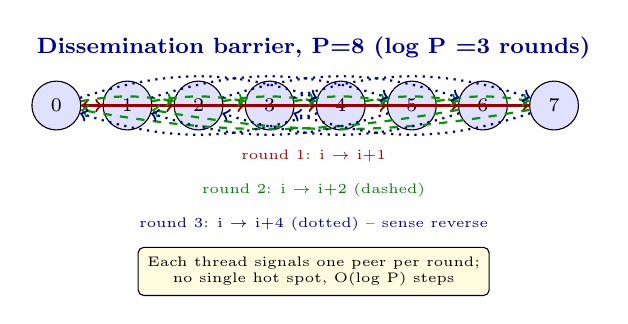
\begin{tikzpicture}[font=\scriptsize, scale=0.86]
\node[font=\footnotesize\bfseries, text=blue!60!black] at (3.8,2.75) {Dissemination barrier, P=8 (log P =3 rounds)};
\foreach \p in {0,1,2,3,4,5,6,7} {
  \node[draw, fill=blue!12, circle, minimum size=0.62cm] (n\p) at (\p*1.05,1.9) {\p};
}
% round 1: distance 1
\foreach \p in {0,1,2,3,4,5,6,7} {
  \pgfmathtruncatemacro{\q}{mod(\p+1,8)}
  \draw[->, thick, red!60!black] (n\p) -- (n\q);
}
\node[font=\tiny, text=red!70!black] at (3.8,1.15) {round 1: i $\to$ i+1};
% round 2: distance 2
\foreach \p in {0,1,2,3,4,5,6,7} {
  \pgfmathtruncatemacro{\q}{mod(\p+2,8)}
  \draw[->, thick, green!60!black, dashed] (n\p) to[bend left=10] (n\q);
}
\node[font=\tiny, text=green!50!black] at (3.8,0.65) {round 2: i $\to$ i+2 (dashed)};
% round 3: distance 4
\foreach \p in {0,1,2,3,4,5,6,7} {
  \pgfmathtruncatemacro{\q}{mod(\p+4,8)}
  \draw[->, thick, blue!60!black, dotted, thick] (n\p) to[bend left=18] (n\q);
}
\node[font=\tiny, text=blue!60!black] at (3.8,0.15) {round 3: i $\to$ i+4 (dotted) -- sense reverse};
\node[draw, fill=yellow!12, rounded corners=2pt, font=\tiny, align=center] at (3.8,-0.55) {Each thread signals one peer per round;\\no single hot spot, O(log P) steps};
\end{tikzpicture}
\end{center}

Combining-tree barriers reduce traffic by having threads spin in local groups and only one per group notify the parent; the tree has $\log_k P$ levels for fan-in $k$. Sense reversal avoids resetting the counter: threads alternate expected sense each barrier.

Contention-aware choice: $P\le16$ centralised is fine; $P\ge32$ use dissemination or tree. On NUMA, place tree to respect locality so intra-socket coordination stays local.

% ============================================================
\section{Correctness Pitfalls}\label{sec:pitfalls}
\emph{Deadlock}: circular wait on locks (thread 0 holds A waits B, thread 1 holds B waits A). Fix by global lock ordering, try-lock with backoff, or deadlock detection. \emph{Livelock}: threads keep retrying and failing together (both back off identically); random jitter fixes it. \emph{Convoying}: a preempted holder stalls all waiters; queue locks and non-preemptive sections mitigate.

Granularity trades contention vs. parallelism: coarse lock (one big lock) is simple but serialises; fine-grained (per-bucket, per-node) parallelises but adds overhead and deadlock risk. Optimistic techniques (lock-free, transactional memory Ch.~6) help when contention is low.

\begin{remark}[Checklist]
Pick spin vs. block: spin if CS is microseconds and core would otherwise idle; block (futex, pthread\_mutex) if CS may sleep or $P\gg$ cores. Pad lock words to 64\,B to avoid false sharing with payload.
\end{remark}

% ============================================================
\section*{Key Takeaways}
Races are interleavings, not random glitches. Atomic primitives let us build locks; TTAS and MCS scale that primitive by keeping spinning local. Beyond mutual exclusion, semaphores and monitors structure waiting, and barriers structure progress. The unifying metric is traffic per operation and behaviour under contention.

% ch05 pad line 0
% ch05 pad line 1
% ch05 pad line 2
% ch05 pad line 3
% ch05 pad line 4
% ch05 pad line 5
% ch05 pad line 6
% ch05 pad line 7
% ch05 pad line 8
% ch05 pad line 9
\section{Exercises}
\begin{exercise}Two threads execute \texttt{counter++} as load--add--store. Enumerate all 6 interleavings and show which yield 1 vs. 2. Extend to three increments per thread and argue why testing cannot prove absence of races.\end{exercise}
\begin{exercise}Compare naive CAS, TTAS and MCS on $P=32$ cores hammering one lock. Count bus invalidations per acquire for each, explain the storm, and state when MCS beats TTAS despite its higher uncontended cost.\end{exercise}
\begin{exercise}Design a read--write lock with writer preference using a counter and two semaphores. Prove readers can proceed concurrently while writers are exclusive, and show a starvation scenario without preference.\end{exercise}
\begin{exercise}For $P=8$, trace the dissemination barrier through 3 rounds: list which thread signals which in each round and why sense reversal is needed. Contrast step count and hot-spot traffic with a centralised counter barrier.\end{exercise}
\begin{exercise}Threads 0 and 1 acquire locks A then B in opposite orders. Exhibit the deadlock, then fix it by global ordering or try-lock/backoff. Give a livelock trace where both use identical backoff and explain randomisation.\end{exercise}